\documentclass[tikz,border=10pt]{standalone}
\usetikzlibrary{shapes.geometric, arrows.meta, positioning, calc, backgrounds}

\begin{document}
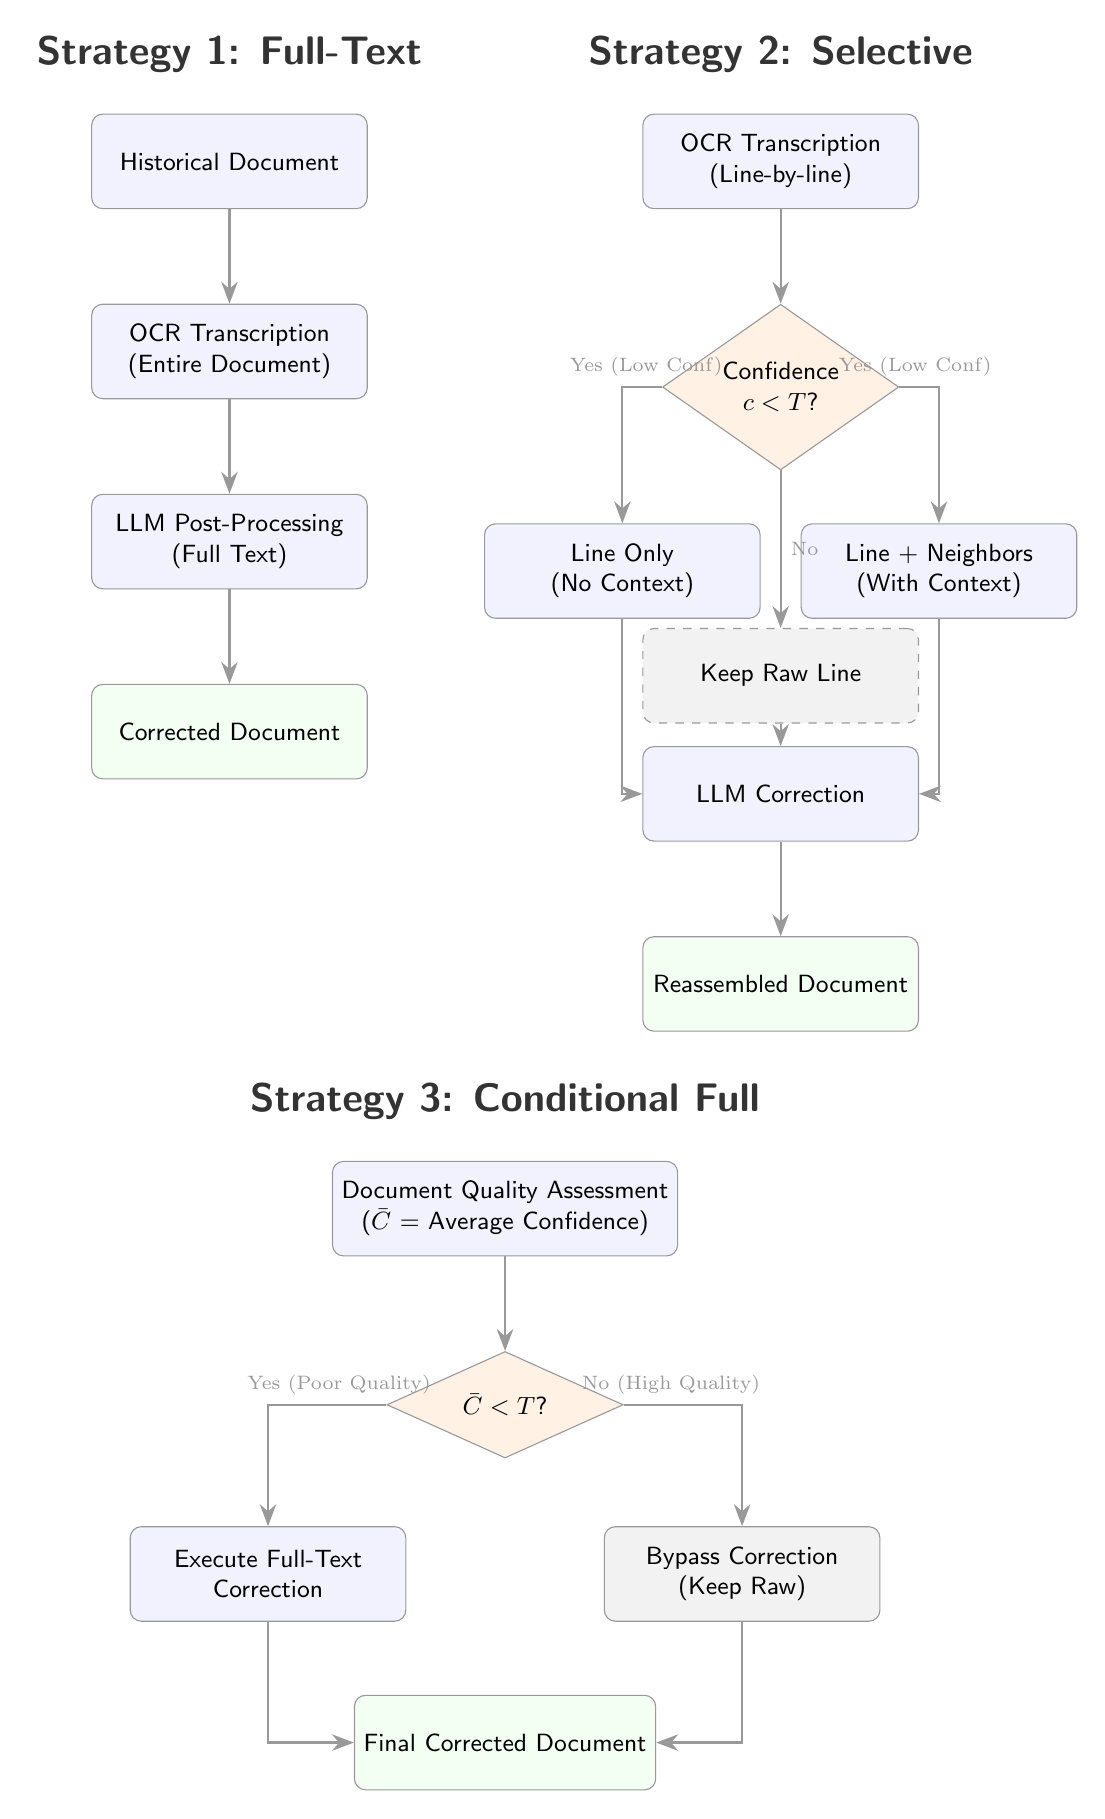
\begin{tikzpicture}[
    node distance=1.2cm and 1.5cm,
    box/.style={rectangle, draw=gray!80, fill=blue!5, rounded corners, minimum width=3.5cm, minimum height=1.2cm, align=center, font=\small\sffamily},
    decision/.style={diamond, draw=gray!80, fill=orange!10, minimum width=3cm, minimum height=1.2cm, align=center, font=\small\sffamily, inner sep=0pt},
    arrow/.style={-{Stealth[scale=1.2]}, thick, gray!80},
    title/.style={font=\Large\bfseries\sffamily, color=black!80},
    label/.style={font=\scriptsize\sffamily, color=gray!80}
]

% Strategy 1: Full-Text
\node[title] (s1) at (0,0) {Strategy 1: Full-Text};
\node[box, below=0.4cm of s1] (s1_doc) {Historical Document};
\node[box, below=of s1_doc] (s1_ocr) {OCR Transcription\\(Entire Document)};
\node[box, below=of s1_ocr] (s1_llm) {LLM Post-Processing\\(Full Text)};
\node[box, below=of s1_llm, fill=green!5] (s1_out) {Corrected Document};

\draw[arrow] (s1_doc) -- (s1_ocr);
\draw[arrow] (s1_ocr) -- (s1_llm);
\draw[arrow] (s1_llm) -- (s1_out);

% Strategy 2: Selective
\node[title] (s2) at (7cm, 0) {Strategy 2: Selective};
\node[box, below=0.4cm of s2] (s2_ocr) {OCR Transcription\\(Line-by-line)};
\node[decision, below=of s2_ocr] (s2_conf) {Confidence \\ $c < T$?};

% Branches for Strategy 2
\node[box, below left=1.2cm and -0.5cm of s2_conf] (s2_noctx) {Line Only\\(No Context)};
\node[box, below right=1.2cm and -0.5cm of s2_conf] (s2_ctx) {Line + Neighbors\\(With Context)};
\node[box, below=2cm of s2_conf, fill=gray!10, dashed] (s2_keep) {Keep Raw Line};

\node[box, below=3.5cm of s2_conf] (s2_llm) {LLM Correction};
\node[box, below=of s2_llm, fill=green!5] (s2_out) {Reassembled Document};

\draw[arrow] (s2_ocr) -- (s2_conf);
\draw[arrow] (s2_conf.west) -| node[above, pos=0.2, font=\scriptsize] {Yes (Low Conf)} (s2_noctx);
\draw[arrow] (s2_conf.east) -| node[above, pos=0.2, font=\scriptsize] {Yes (Low Conf)} (s2_ctx);
\draw[arrow] (s2_conf) -- node[right, font=\scriptsize] {No} (s2_keep);

\draw[arrow] (s2_noctx) |- (s2_llm);
\draw[arrow] (s2_ctx) |- (s2_llm);
\draw[arrow] (s2_keep) -- (s2_llm);
\draw[arrow] (s2_llm) -- (s2_out);


% Strategy 3: Conditional Full
\node[title] (s3) at (3.5cm, -13.3cm) {Strategy 3: Conditional Full};
\node[box, below=0.4cm of s3] (s3_doc) {Document Quality Assessment\\($\bar{C}$ = Average Confidence)};
\node[decision, below=of s3_doc] (s3_check) {$\bar{C} < T$?};

\node[box, below left=1.2cm and 0.5cm of s3_check] (s3_full) {Execute Full-Text\\Correction};
\node[box, below right=1.2cm and 0.5cm of s3_check, fill=gray!10] (s3_bypass) {Bypass Correction\\(Keep Raw)};

\node[box, below=3cm of s3_check, fill=green!5] (s3_out) {Final Corrected Document};

\draw[arrow] (s3_doc) -- (s3_check);
\draw[arrow] (s3_check.west) -| node[above, pos=0.2, font=\scriptsize] {Yes (Poor Quality)} (s3_full);
\draw[arrow] (s3_check.east) -| node[above, pos=0.2, font=\scriptsize] {No (High Quality)} (s3_bypass);

\draw[arrow] (s3_full) |- (s3_out);
\draw[arrow] (s3_bypass) |- (s3_out);

\end{tikzpicture}
\end{document}
